% Author: Alfredo Sánchez Alberca (asalber@ceu.es)
% !TEX program = xelatex
%----------------------------------------------------------------------------------------
%    DOCUMENT CLASS
%----------------------------------------------------------------------------------------

\documentclass[11pt,a4paper,openright]{book}
%----------------------------------------------------------------------------------------
%	PACKAGES AND OTHER DOCUMENT CONFIGURATIONS
%----------------------------------------------------------------------------------------

% Language settings
\usepackage{polyglossia}
\setdefaultlanguage{english}

% Margins and layout
\usepackage[top=3cm, bottom=3cm, left=2.54cm, right=2.54cm]{geometry}

% Math support
\usepackage{amsmath, amssymb}
% \usepackage{mathspec}

% Font settings
\usepackage{unicode-math}
\setmainfont[Ligatures=TeX]{TeX Gyre Pagella}
\setmathfont{TG Pagella Math}
% \setmathfont[math-style=ISO, bold-style=ISO]{texgyrepagella-math.otf}

% Color
\usepackage{xcolor} % Required for specifying colors by name
\definecolor{color1}{RGB}{5,161,230}
\definecolor{color2}{RGB}{238,50,36}
\definecolor{ocre}{RGB}{243,102,25} % Define the orange color used for highlighting throughout the book
\definecolor{blueceu}{RGB}{5,161,230} % Blue color of CEU logo
\definecolor{greenceu}{RGB}{185,209,16} % Green color of CEU logo
\definecolor{redceu}{RGB}{238,50,36} % Red color of CEU logo
\definecolor{grayceu}{RGB}{111,107,83} % Gray color of CEU logo
\definecolor{coral}{rgb}{1,0.5,0.31} % Orange color for graphics
\definecolor{royalblue1}{rgb}{0.28,0.46,1} % Blue color for graphics
\definecolor{mygreen}{rgb}{0,0.8,0} % Green color for graphics
\definecolor{chaptergrey}{RGB}{5,161,230} % Blue color of CEU logo

% Line breaking
\usepackage{microtype} 
\setlength{\emergencystretch}{2em}

% Graphics
\usepackage{graphicx}
\usepackage{tikz} 
\usepackage{eso-pic} % Required for specifying an image background in the title page

% Arrays and tables
\usepackage{array}
\usepackage{multirow}
\usepackage{colortbl}
\usepackage{booktabs}
\newcommand{\tcrule}{\arrayrulecolor{color1!50!white}\toprule}
\newcommand{\mcrule}{\arrayrulecolor{color1!50!white}\midrule}
\newcommand{\bcrule}{\arrayrulecolor{color1!50!white}\bottomrule}

% Captions
\usepackage[margin=20pt, font=small, labelfont=bf, labelsep=endash]{caption}

% Floating figures
\usepackage{subfigure}

% Lists
\usepackage[shortlabels]{enumitem} % Customize lists
%\setlist{nolistsep} % Reduce spacing between bullet points and numbered lists
\setlist[description]{style=sameline,leftmargin=0cm}

% Columns
\usepackage{multicol}

% Creative common icons
\usepackage[scale=2]{ccicons}

% \makeatletter
% \let\savees@listquot\es@listquot
% \def\es@listquot{\protect\savees@listquot}
% \makeatletter

% hyperlinks
\usepackage{hyperref}
\hypersetup{
pdfauthor = {Alfredo S\'anchez Alberca},
pdftitle = {Calculus practices with Geogebra},
pdfsubject = {Calculus},
pdfkeywords = {Mathematics, Calculus, Geogebra},
pdfcreator = {XeLaTeX with hyperref package},
pdfproducer = {pdfLaTeX},
colorlinks = true,
linkcolor = red,          % color of internal links
citecolor = green,        % color of links to bibliography
filecolor = magenta,      % color of file links
urlcolor = magenta,          % color of external links
}
%\usepackage{breakurl}

% Indentation
%\setlength\parindent{0pt}

% Control of widow orphan lines
\clubpenalty=10000
\widowpenalty=10000 

%Code listing formatting
\usepackage{listings}
\lstdefinelanguage{morejava}{morekeywords={String}}
\definecolor{vollgrau}{rgb}{0.9,0.9,0.9}
\definecolor{colKeys}{rgb}{0,0,1}
\definecolor{colIdentifier}{rgb}{0,0,0}
\definecolor{colComments}{rgb}{1,0.5,0}
\definecolor{colString}{rgb}{0,0.5,0}
\definecolor{colbackground}{rgb}{0.9,0.9,1}
\lstset{%
      language=R,
      float=hbp,%
      basicstyle=\ttfamily,%
      identifierstyle=\color{colIdentifier},%
      keywordstyle=\color{colKeys},%
      stringstyle=\color{colString},%
      commentstyle=\color{colCommentsxelatex},%
%    columns=flexible,%xelatex
%    columns=fullflexible,%xelatex
      columns=fixed, %xelatex
      tabsize=1,%xelatex
      extendedchars=true,%xelatex
      showspaces=false,%xelatex
      showstringspaces=false,%xelatex
      breaklines=true,%xelatex
      breakindent=10pt,%xelatex
      backgroundcolor=\color{colbackgxelatexround},%
      breakautoindent=true,%xelatex
      captionpos=t,%
      xleftmargin=1em,%
%    xrightmargin=.5\fboxsep,%
      numbersep=1em,%
      escapechar=\#\RequirePackage[\eu@zf@math]{fontspec}[2008/08/09]
}

% Set short or lon\RequirePackage[\eu@zf@math]{fontspec}[2008/08/09]ersion desired
% \usepackage[cort\RequirePackage[\eu@zf@math]{fontspec}[2008/08/09]

%----------------------------------------------------------------------------------------
%	SECTIONS AND SUBSECTIONS
%----------------------------------------------------------------------------------------
%\titleformat*{\section}{\Huge}
%\titleformat*{\subsection}{\Large}


% Chapter and section formatting 
\usepackage[rigidchapters,explicit]{titlesec}
\setlength{\fboxsep}{5pt}
\newlength{\titulolength}
\setlength{\titulolength}{\textwidth} 
\addtolength{\titulolength}{-2\fboxsep}
\addtolength{\titulolength}{-2\fboxrule}
\titleformat{\chapter}[display]
{\bfseries\sffamily}
{\filleft \mdseries \LARGE \color{blueceu} Practice \Huge\thechapter}
{0.5ex}
{\colorbox{blueceu}{\parbox[t]{\titulolength}{\rule{0mm}{10mm}\Huge\sffamily\filleft\textcolor{white}{#1}}}}
\titleformat{\section}{\normalfont\Large\bfseries\color{blueceu}}{\arabic{section}}{1em}{#1}
\titleformat{\subsection}{\normalfont\large\bfseries\color{blueceu}}{\arabic{section}.\arabic{subsection}}{1em}{#1}
\titleformat{\subsubsection}{\normalfont\normalsize\bfseries\color{blueceu}}{\arabic{section}.\arabic{subsection}.\arabic{subsubsection}}{0.5em}{#1}
\titlespacing{\chapter}{0pt}{0pt}{30ex}
\titlespacing{\section}{0pt}{8ex}{4ex}

%----------------------------------------------------------------------------------------
%	MAIN TABLE OF CONTENTS
%----------------------------------------------------------------------------------------

% \usepackage{titletoc} % Required for manipulating the table of contents
% 
% \contentsmargin{0cm} % Removes the default margin
% % Chapter text styling
% \titlecontents{chapter}[1.25cm] % Indentation
% {\addvspace{15pt}\large\bfseries} % Spacing and font options for chapters
% {\color{gray}\contentslabel[\Large\thecontentslabel.]{1.25cm}} % Chapter number
% {}  
% {\color{gray}\bfseries\hfill\thecontentspage} % Page number
% % Section text styling
% \titlecontents{section}[1.25cm] % Indentation
% {\addvspace{5pt}\bfseries} % Spacing and font options for sections
% {\contentslabel[\thecontentslabel]{1.25cm}} % Section number
% {}
% {\hfill\color{black}\thecontentspage} % Page number
% []
% % Subsection text styling
% \titlecontents{subsection}[1.25cm] % Indentation
% {\addvspace{1pt}\small} % Spacing and font options for subsections
% {\contentslabel[\thecontentslabel]{1.25cm}} % Subsection number
% {}
% {\;\titlerule*[.5pc]{.}\;\thecontentspage} % Page number
% [] 

%----------------------------------------------------------------------------------------
%	MINI TABLE OF CONTENTS IN CHAPTER HEADS
%----------------------------------------------------------------------------------------

% % Section text styling
% \titlecontents{lsection}[0em] % Indendating
% {\footnotesize\sffamily} % Font settings
% {}
% {}
% {}
% 
% % Subsection text styling
% \titlecontents{lsubsection}[.5em] % Indentation
% {\normalfont\footnotesize\sffamily} % Font settings
% {}
% {}
% {}
 
%----------------------------------------------------------------------------------------
%	PAGE HEADERS
%----------------------------------------------------------------------------------------

% Headings and footers
\usepackage{fancyhdr}
\pagestyle{fancy}
\fancyhead{}
\renewcommand{\chaptermark}[1]{\markboth{\thechapter.\ #1}{}}
\fancyhead[LE]{\scshape Matemática Aplicada con Geogebra}
\fancyhead[RO]{\sffamily\slshape \leftmark}
\renewcommand{\headrulewidth}{0pt}
\renewcommand{\floatpagefraction}{.8}
\renewcommand{\textfraction}{.1}


% \usepackage{fancyhdr} % Required for header and footer configuration
% 
% \pagestyle{fancy}
% \renewcommand{\chaptermark}[1]{\markboth{\color{grayceu}\sffamily\normalsize\textit{#1}}{}} % Chapter text font
% % settings
% %\renewcommand{\sectionmark}[1]{\markright{\color{grayceu}\sffamily\normalsize\textit{\thesection\hspace{5pt}#1}}{}} %
% % Section text font settings
% \fancyhf{} \fancyfoot[LE,RO]{\normalsize\thepage} % Font setting for the page number in the footer
% \fancyhead[RE]{{\color{grayceu}\sffamily\normalsize\textit{Pr�cticas de Bioestad�stica con R and RKTeaching}}} % Print the nearest
% % section name on the left side of odd pages
% \fancyhead[LO]{\leftmark} % Print the current chapter name on the right side of even pages
% \renewcommand{\headrulewidth}{0pt} % Removes the rule in the header
% \addtolength{\headheight}{2.5pt} % Increase the spacing around the header slightly
% \renewcommand{\footrulewidth}{0pt} % Removes the rule in the footer
% \fancypagestyle{plain}{\fancyhead{}\renewcommand{\headrulewidth}{0pt}} % Style for when a plain pagestyle is specified
% 
% % Removes the header from odd empty pages at the end of chapters
% \makeatletter
% \renewcommand{\cleardoublepage}{
% \clearpage\ifodd\c@page\else
% \hbox{}
% \vspace*{\fill}
% \thispagestyle{empty}
% \newpage
% \fi}


%----------------------------------------------------------------------------------------
%	THEOREM STYLES
%----------------------------------------------------------------------------------------

\usepackage{amsthm} % For including math equations, theorems, symbols, etc

\newcommand{\intoo}[2]{\mathopen{]}#1\,;#2\mathclose{[}}
\newcommand{\ud}{\mathop{\mathrm{{}d}}\mathopen{}}
\newcommand{\intff}[2]{\mathopen{[}#1\,;#2\mathclose{]}}
\newtheorem{notation}{Notación}[chapter]

\newtheoremstyle{blueceu} % Theorem style name
{7pt} % Space above
{7pt} % Space below
{\normalfont} % Body font
{} % Indent amount
{\small\bf\sffamily\color{blueceu}} % Theorem head font
{\;\;} % Punctuation after theorem head
{0.25em} % Space after theorem head
{\small\sffamily\color{blueceu}\thmname{#1}\thmnumber{\@ifnotempty{#1}{ }\@upn{#2}} % Theorem text (e.g. Theorem 2.1)
\thmnote{\ {\the\thm@notefont\sffamily\bfseries\color{blueceu}--- #3.}}} % Optional theorem note
\renewcommand{\qedsymbol}{$\blacksquare$} % Optional qed square

\newtheoremstyle{blacknumex} % Theorem style name
{7pt} % Space above
{7pt} % Space below
{\normalfont} % Body font
{} % Indent amount
{\small\bf\sffamily} % Theorem head font
{\;\;} % Punctuation after theorem head
{0.25em} % Space after theorem head
{\small\sffamily{\tiny\ensuremath{\blacksquare}}\ \thmname{#1}\thmnumber{\@ifnotempty{#1}{ }\@upn{#2}} % Theorem text (e.g. Theorem 2.1)
\thmnote{\ {\the\thm@notefont\sffamily\bfseries--- #3.}}} % Optional theorem note

\newtheoremstyle{blacknum} % Theorem style name
{7pt} % Space above
{7pt} % Space below
{\normalfont} % Body font
{} % Indent amount
{\small\bf\sffamily} % Theorem head font
{\;\;} % Punctuation after theorem head
{0.25em} % Space after theorem head
{\small\sffamily\thmname{#1}\thmnumber{\@ifnotempty{#1}{ }\@upn{#2}} % Theorem text (e.g. Theorem 2.1)
\thmnote{\ {\the\thm@notefont\sffamily\bfseries--- #3.}}} % Optional theorem note

\newtheoremstyle{example} % Theorem style name
{7pt} % Space above
{7pt} % Space below
{\normalfont} % Body font
{} % Indent amount
{\small\bf\sffamily} % Theorem head font
{\;\;} % Punctuation after theorem head
{0.25em} % Space after theorem head
{\small\sffamily\thmname{#1} % Theorem text (e.g. Theorem 2.1)
\thmnote{\ {\the\thm@notefont\sffamily\bfseries--- #3.}}} % Optional theorem note

\newtheoremstyle{indication} % Theorem style name
{-5pt} % Space above
{7pt} % Space below
{\normalfont} % Body font
{-28pt} % Indent amount
{\bf} % Theorem head font
{\kern-11.5pt} % Punctuation after theorem head
{20pt} % Space after theorem head
{\begin{tikzpicture}
\draw node [fill=blueceu,opacity=1,inner sep=1pt] {\makebox[17pt][c]{
\includegraphics[scale=0.3]{img/bulb}}}; \end{tikzpicture}} % Theorem text (e.g. Theorem 2.1)

\makeatother

% Defines the theorem text style for each type of theorem to one of the three styles above
\theoremstyle{ocrenum}
\newtheorem{exerciseT}{Exercise}[chapter]
\theoremstyle{blacknumex}
\newtheorem{exampleT}{Example}[chapter]
%\theoremstyle{blacknum}
\theoremstyle{blueceu}
\newtheorem{vocabulary}{Vocabulario}[chapter]
\newtheorem{definitionT}{Definición}[chapter]
\newtheorem{theoremT}{Teorema}[chapter]
\newtheorem{corolary}{Corolario}[chapter]
\theoremstyle{indication}
\newtheorem{indicationT}{Indicación}
%\theoremstyle{example}
%\newtheorem{ejemplo}{Ejemplo}

%----------------------------------------------------------------------------------------
%	DEFINITION OF COLORED BOXES
%----------------------------------------------------------------------------------------

\RequirePackage[framemethod=default]{mdframed} % Required for creating the theorem, definition, exercise and corollary boxes

% Theorem box
\newmdenv[skipabove=7pt,
skipbelow=7pt,
backgroundcolor=black!5,
linecolor=ocre,
innerleftmargin=5pt,
innerrightmargin=5pt,
innertopmargin=5pt,
leftmargin=0cm,
rightmargin=0cm,
innerbottommargin=5pt]{tBox}

% Exercise box	  
\newmdenv[skipabove=7pt,
skipbelow=7pt,
rightline=false,
leftline=true,
topline=false,
bottomline=false,
backgroundcolor=ocre!10,
linecolor=ocre,
innerleftmargin=5pt,
innerrightmargin=5pt,
innertopmargin=5pt,
innerbottommargin=5pt,
leftmargin=0cm,
rightmargin=0cm,
linewidth=4pt]{eBox}	

% Definition box
\newmdenv[skipabove=10pt,
skipbelow=10pt,
rightline=false,
leftline=true,
topline=false,
bottomline=false,
linecolor=ocre,
innerleftmargin=5pt,
innerrightmargin=5pt,
innertopmargin=0pt,
leftmargin=0cm,
rightmargin=0cm,
linewidth=4pt,
innerbottommargin=0pt]{dBox}	

% Corollary box
\newmdenv[skipabove=7pt,
skipbelow=7pt,
rightline=false,
leftline=true,
topline=false,
bottomline=false,
linecolor=gray,
backgroundcolor=black!5,
innerleftmargin=5pt,
innerrightmargin=5pt,
innertopmargin=5pt,
leftmargin=0cm,
rightmargin=0cm,
linewidth=4pt,
innerbottommargin=5pt]{cBox}	

% Indication box
\newmdenv[skipabove=7pt,
skipbelow=7pt,
rightline=false,
leftline=true,
topline=false,
bottomline=false,
linecolor=blueceu,
backgroundcolor=black!5,
innerleftmargin=5pt,
innerrightmargin=5pt,
innertopmargin=5pt,
leftmargin=0pt,
rightmargin=0pt,
linewidth=4pt,
innerbottommargin=5pt]{iBox}		  
		  			  


% Creates an environment for each type of theorem and assigns it a theorem text style from the "Theorem Styles" section above and a colored box from above
\newenvironment{theorem}{\begin{tBox}\begin{theoremT}}{\end{theoremT}\end{tBox}}
\newenvironment{exercise}{\begin{eBox}\begin{exerciseT}}{\hfill{\color{ocre}\tiny\ensuremath{\blacksquare}}\end{exerciseT}\end{eBox}}				  
\newenvironment{definition}{\begin{dBox}\begin{definitionT}}{\end{definitionT}\end{dBox}}	
\newenvironment{example}{\begin{exampleT}}{\hfill{\tiny\ensuremath{\blacksquare}}\end{exampleT}}		
\newenvironment{corollary}{\begin{cBox}\begin{corollaryT}}{\end{corollaryT}\end{cBox}}	
\newenvironment{indication}{\begin{iBox}\begin{indicationT} \renewcommand{\theenumii}{\arabic{enumii}}\renewcommand{\labelenumii}{\sffamily\theenumii)}\renewcommand{\theenumiii}{\arabic{enumiii}}\renewcommand{\labelenumiii}{\sffamily\theenumiii)}}{\end{indicationT}\end{iBox}}	

%----------------------------------------------------------------------------------------
%	REMARK ENVIRONMENT
%----------------------------------------------------------------------------------------

%\newenvironment{remark}{\par\vskip10pt\small % Vertical white space above the remark and smaller font size
%\begin{list}{}{
%\leftmargin=35pt % Indentation on the left
%\rightmargin=25pt}\item\ignorespaces % Indentation on the right
%\makebox[-2.5pt]{\begin{tikzpicture}[overlay]
%\node[draw=ocre!60,line width=1pt,circle,fill=ocre!25,font=\sffamily\bfseries,inner sep=2pt,outer sep=0pt] at (-15pt,0pt){\textcolor{ocre}{R}};\end{tikzpicture}} % Orange R in a circle
%\advance\baselineskip -1pt}{\end{list}\vskip5pt} % Tighter line spacing and white space after remark

% %----------------------------------------------------------------------------------------
% %	SECTION NUMBERING IN THE MARGIN
% %----------------------------------------------------------------------------------------
% 
% \makeatletter
% %\renewcommand{\@seccntformat}[1]{\llap{\textcolor{grayceu}{\csname the#1\endcsname.}\hspace{1em}}}                    
% \renewcommand{\section}{
% 	\@startsection{section}{1}{\z@}
% 	{-4ex \@plus -1ex \@minus -.4ex}{1ex \@plus.2ex }
% 	{\normalfont\LARGE}
% }
% \renewcommand{\subsection}{
% 	\@startsection{subsection}{2}{\z@}
% 	{-3ex \@plus -0.1ex \@minus -.4ex}{0.5ex \@plus.2ex }
% 	{\normalfont\Large}
% }
% \renewcommand{\subsubsection}{
% 	\@startsection{subsubsection}{3}{\z@}
% 	{-2ex \@plus -0.1ex \@minus -.2ex}{0.2ex \@plus.2ex }
% 	{\normalfont\large}
% }                        
% \renewcommand{\paragraph}{
% 	\@startsection{paragraph}{4}{\z@}
% 	{-2ex \@plus-.2ex \@minus .2ex}{0.1ex}
% 	{\normalfont\bfseries}
% }
% 
% \def\thechapter{\arabic{chapter}}
% \def\thesection{\thechapter.\arabic{section}.}
% \def\thesubsection{\thesection\arabic{subsection}.}
% \def\thesubsubsection{\thesubsection\arabic{section}.}
% 
% %----------------------------------------------------------------------------------------
% %	CHAPTER HEADINGS
% %----------------------------------------------------------------------------------------
% %\newcommand{\thechapterimage}{}
% %\newcommand{\chapterimage}[1]{\renewcommand{\thechapterimage}{#1}}
% \def\@makechapterhead#1{
% \thispagestyle{empty}
% {
% \ifnum \c@secnumdepth >\m@ne
% \if@mainmatter
% \startcontents
% \begin{tikzpicture}[remember picture,overlay]
% % \node at (current page.north west)
% % {\begin{tikzpicture}[remember picture,overlay]
% % 
% % %\node[anchor=north west] at (-4pt,-27.5mm) {\includegraphics[width=\paperwidth]{\thechapterimage}};
% % %Commenting the 3 lines below removes the small contents box in the chapter heading
% % % \draw[fill=white,opacity=.6] (30mm,-30mm) rectangle (9cm,-9cm);
% % % \node[anchor=north west] at (30mm,-30mm) {\parbox[t][9cm][t]{5.5cm}{\huge\bfseries\flushleft \printcontents{l}{1}{\setcounter{tocdepth}{2}}}};
% % % \draw[anchor=west] (5cm,-11cm) node [rounded corners=25pt,fill=white,opacity=.7,inner sep=15.5pt]{\huge\sffamily\bfseries\textcolor{black}{\vphantom{plPQq}\makebox[20cm]{}}};
% \draw[anchor=north west, fill=black] (0mm,50mm) rectangle (1pt,10mm);
% \draw[anchor=north west] (0cm,20mm) node {\scalebox{1.5}{\Huge{\textcolor{grayceu}\thechapter}}}; 
% %\draw[anchor=west] (0cm,0cm) node {\Huge{#1}}; 
% \end{tikzpicture}
% \par\vspace*{2cm}
% {\Huge #1}
% \par\vspace*{1cm}
% % \end{tikzpicture}}\par\vspace*{230\p@}
% }}
% \def\@makeschapterhead#1{
% \thispagestyle{empty}
% {
% \ifnum \c@secnumdepth >\m@ne
% \if@mainmatter
% \startcontents
% \begin{tikzpicture}[remember picture,overlay]
% % \node at (current page.north west)
% % {\begin{tikzpicture}[remember picture,overlay]
% % \node[anchor=north west] at (-4pt,-27.5mm) {\includegraphics[width=\paperwidth]{\thechapterimage}};
% % \draw[anchor=west] (5cm,-11cm) node [rounded corners=25pt,fill=white,opacity=.7,inner sep=15.5pt]{\huge\sffamily\bfseries\textcolor{black}{\vphantom{plPQq}\makebox[20cm]{}}};
% % \draw[anchor=west] (5cm,-11cm) node [rounded corners=25pt,inner sep=15.5pt]{\huge\sffamily\bfseries\textcolor{black}{#1\vphantom{plPQq}\makebox[20cm]{}}};
% % \end{tikzpicture}};
% % \end{tikzpicture}}\par\vspace*{230\p@}
% %\draw[anchor=west] (0cm,0cm) node {\Huge{#1}}; 
% \end{tikzpicture}
% {\Huge #1}
% \par\vspace*{1cm}
% }}
% \makeatother

 % Insert the commands_book.tex file which contains the majority of the structure behind
% the template

%----------------------------------------------------------------------------------------
%	COMMANDS FOR INDICATIONS
%----------------------------------------------------------------------------------------
\usepackage{menukeys}
\DeclareFontFamily{\encodingdefault}{\ttdefault}{\hyphenchar\font=`\-}
\newmenucolortheme{mycolors}{named}{white}{color1}{black}
\changemenucolortheme{menus}{mycolors}
\renewmenumacro{\menu}[>]{menus}
%\newmenustylesimple*{botonstyle}{\textbf{\CurrentMenuElement}}
%\renewmenumacro{\keys}{botonstyle}
\newcommand{\button}[1]{\textsf{\small #1}}
\newcommand{\option}[1]{\textsf{\small #1}}
\newcommand{\mtab}[1]{\textsf{\small #1}}
\newcommand{\field}[1]{\textsf{\small #1}}
\newcommand{\command}[1]{\texttt{#1}}
\newcommand{\variable}[1]{\textsf{\small #1}}
\newcommand{\result}[1]{\texttt{#1}}

% OTHERS
\newcommand{\resetcounters}{\setcounter{page}{1} \setcounter{section}{0} \setcounter{footnote}{0} \setcounter{figure}{0} \setcounter{table}{0}}

%========================================================================================
%   DOCUMENT BODY
%========================================================================================
\begin{document}
\frontmatter
% Add two blank pages at the begining
%\null\thispagestyle{empty}\newpage
%\null\thispagestyle{empty}\newpage
%----------------------------------------------------------------------------------------
%	TITLE PAGE
%----------------------------------------------------------------------------------------
\begin{titlepage}
\thispagestyle{empty}
\vspace*{7cm}
\par

% Book title
\begin{center}
\normalfont\fontsize{30}{30}\selectfont
{\bfseries \color{blueceu}Calculus with Geogebra}
\end{center}
\vspace{1cm}

% Authors names
\begin{center}
\Large
\begin{tabular}{c}
Edgar Arribas Gimeno (\url{edgar.arribasgimeno@ceu.es})\\
Juan Carlos Garro Garro (\url{garro.eps@ceu.es})\\
Alfredo Sánchez Alberca (\url{asalber@ceu.es})\\
Alberto Zaragoza de Lorite (\url{alberto.zaragozalorite@ceu.es})
\end{tabular}

\medskip 
Department of Maths and Data Science\\ CEU San Pablo University\\[1cm]
\medskip 
September 2022

\vspace{1cm}

\includegraphics[height=3cm]{img/logo_uspceu}
\end{center}
\vfill
\end{titlepage}
%\input{preamble/titlepage_book} 

%----------------------------------------------------------------------------------------
%	COPYRIGHT PAGE
%----------------------------------------------------------------------------------------
\thispagestyle{empty}
\null
\vfill
\hrule depth 3pt
\smallskip
\sffamily

\noindent \textbf{Calculus with Geogebra}\\
Alfredo Sánchez Alberca (asalber@ceu.es) 

\bigskip
% Creative Commons license terms
{\Large \textbf{License terms \normalsize \ccLogo}}
\medskip

\small
This work is licensed under an Attribution--NonCommercial--ShareAlike 4.0 International Creative Commons License. 
\url{http://creativecommons.org/licenses/by-nc-sa/4.0/}

You are free to: 

\begin{itemize}
\item \textbf{Share}: Copy and redistribute the material in any medium or format
\item \textbf{Adapt}: Remix, transform, and build upon the material
\end{itemize}

Under the following terms:
\begin{center}
\begin{tabular}{cp{0.8\textwidth}}
\ccAttribution &  \textbf{Attribution}. You must give appropriate credit, provide a link
to the license, and indicate if changes were made. You may do so in any reasonable manner, but not in any way that
suggests the licensor endorses you or your use.\\ 
\ccNonCommercialEU & \textbf{NonComercial}. You may not use the material for commercial purposes.\\ 
\ccShareAlike & \textbf{ShareAlike}. If you remix, transform, or build upon the material, you must distribute
your contributions under the same license as the original.
\end{tabular}
\end{center}

No additional restrictions — You may not apply legal terms or technological measures that legally restrict others from
doing anything the license permits.

\hrule depth 3pt

\normalfont
\newpage

%----------------------------------------------------------------------------------------
%	TABLE OF CONTENTS
%----------------------------------------------------------------------------------------
%\chapterimage{img/chapter_head.png} % Table of contents heading image
{\pagestyle{plain} % No headers
%\input{registro}
\tableofcontents\thispagestyle{empty}
% Print the table of contents itself
\cleardoublepage % Forces the first cxelatexhapter to start on an odd page so it's on the right
}
\mainmatter
%----------------------------------------------------------------------------------------
%	CHAPTERS
%----------------------------------------------------------------------------------------
% !TEX root = ../geogebra-practices.tex
% Author: Alfredo Sánchez Alberca (asalber@ceu.es)
\chapter{Introduction to Geogebra}

\section{Introduction}
In the last decades, the computational power of computers have converted them in powerful tools for disciplines that, as Mathematics, require a large amount of complex computations.

Geogebra\footnote{These practices are based on version 6.0 of Classic Geogebra} is one of the most used programs for doing numerical and symbolic computations.
Beyond their capabilities for the numerical, vectorial and matrix calculus, it also makes graphical representations.
This allows to solve a lot of problems of Algebra, Analysis, Calculus, Geometry and even Statistics.
The advantage of Geogebra versus other software as Mathematica, Mapple or MATLAB, is its simplicity, what makes it suitable for teaching Maths, and that is open source software, so that it can be modified and installed for free.

\begin{center}

\includegraphics[scale=0.8]{img/introduction/geogebra-logo}
\end{center}

This software can be downloaded from the web \url{https://www.geogebra.org}.
There is also in this web an on-line version of the program that can be used as a web application without installing it in the computer.
This web also contains a lot of tutorials an educational resources available to the users.
In fact, any user can register an upload to this site activities developed with Geogebra.

The goal of this practice is to introduce to the student the basic usage of this program for Calculus.


\section{Starting the program}
As any other Windows applications, to start the program you have to click the \menu{Windows start} button and then select \menu{All the programs > Geogera} or simply double click the desktop shortcut icon 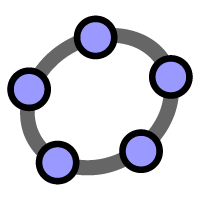
\includegraphics[scale=0.04]{img/introduction/geogebra-icon} if there is one.

When the program starts, the initial windows is shown (figure \ref{g:start-window}), allowing the user to choose among different working environments or \emph{Perspectives}.

\begin{figure}[h!]
\begin{center}
\includegraphics[width=\textwidth]{img/introduction/start-window}
\caption{Starting perspective of Geogegra.} \label{g:start-window}
\end{center}
\end{figure}

\section{Views}
Geogebra provides several windows that are called \emph{Views} and different working environments called \emph{Perspectives} that combine some views.
Both views and perspectives can be activated in the main menu of Geogebra that appears in the top right corner.
The most important views that we are going to use during these practices are:
\begin{description}
\item[Algebraic View] 
\includegraphics[scale=0.03]{img/introduction/algebraic-view-icon} This view allows to make algebraic and geometric constructions.
      It provides an \field{Input Bar} where the user can enter command and algebraic expressions.
      This is view is active by default when the program starts.
\item[Graphic View] 
\includegraphics[scale=0.03]{img/introduction/graphics-view-icon}
      This view allows to represent graphically geometric objects in the real plane.
      Beside the algebraic view, this view is also active by default when the program starts.
\item[3D Graphics View] 
\includegraphics[scale=0.3]{img/introduction/3d-graphics-view-icon} This view allows to represent graphically geometric objects in the real space.
      This view is not activated by default when the program starts, so that it must be activated by the user when it is required.
\item[CAS View] 
\includegraphics[scale=0.03]{img/introduction/cas-view-icon} (Computer Algebra System) This view allows to do symbolic calculations.
      It provides an \field{Input Bar} similar to the one of the algebraic view where you can enter commands and mathematical expressions, and evaluate them.
      This view is not activated by default when the program starts, but \emph{it will be the most used view during these practices}.
\end{description}


\section{Expression edition in the \field{CAS View}}
Before doing any computation with a mathematica expression, you need to know how to enter that expression and learn to manage it.


\subsection*{Entering expressions}
Any mathematical expression must be entered in the \field{Input Bar} of the \field{CAS View} (figure~\ref{g:input-bar}).

\begin{figure}[h!]
\begin{center}

\includegraphics[scale=0.6]{img/introduction/input-bar}
\caption{Input Bar.} \label{g:input-bar}
\end{center}
\end{figure}

The \field{Input Bar} allows to enter mathematical expressions, commands and text annotations.
In the mathematical expressions we can enter numbers, roman letters, greek letters, mathematical operators and any symbols that appears in the virtual keyboard.
It also allows to enter \LaTeX\footnote{\url{https://www.latex-project.org/}} code to format expressions.
For instance, it is possible to write superscripts with the command \command{\^{}} and subscripts with the command \command{\_}.

When the key \command{Enter} is pressed after entering a mathematical expression, Geogebra tries to evaluate it and it shows the result of the evaluation just below the expression, or a warning when there is some mistake in the expression.

Them most common operators for the construction of mathematical expressions are shown in the table below.

\begin{center}
\begin{tabular}{cc}
\tcrule
\textbf{Symbol} & \textbf{Operator} \\
\command{+}     & Addition          \\
\command{-}     & Subtraction       \\
\command{*}     & Product           \\
\command{/}     & Division          \\
\command{\^{}}  & Power             \\
\bcrule
\end{tabular}
\end{center}

At the time of writing a mathematical expression, you must take into account that Geogebra has an order of priority to evaluate the operators.
First it evaluates predefined functions and constants, after powers, after products and quotients (both with the same priority and from left to right), and finally additions and subtractions (both with the same priority and from left to right).
To force the evaluation of a subexpression, skipping the order of priority, you must use parenthesis.
Thus, as it can be appreciated in the table below, depending on how a expression is entered, you can get different results.

\begin{center}\renewcommand{\arraystretch}{2}
\begin{tabular}{cc}
\tcrule
\textbf{Entered expression} & \textbf{Evaluated expression} \\
\texttt{4x-1/x-5}           & $4x-\dfrac{1}{x}-5$           \\
\texttt{(4x-1)/x-5}         & $\dfrac{4x-1}{x}-5$           \\
\texttt{4x-1/(x-5)}         & $4x-\dfrac{1}{x-5}$           \\
\texttt{(4x-1)/(x-5)}       & $\dfrac{4x-1}{x-5}$           \\
\bcrule
\end{tabular}
\end{center}

Every expression that is entered in the \field{CAS View} is labelled with a number that allows to identify it.
Later, every time that we want to reference that expression we can use that identifier instead of writing again the whole expression.

There are two ways of referring to an expression, that are the static and the dynamic references.
To do a static reference we must write the symbol \# followed by the identifier number of the expression.
On the other hand, to do a dynamic reference we must write the symbol \$ followed by the identifier number of the expression.
A static reference will not change the expression where the reference is done even when the original expression changes, while for a dynamic reference, when the original expression changes, that change will be reflected in the expression where the reference is done.

It is possible to select any expression or subexpression of the \field{CAS View} and then copy and paste it in the \field{Input Bar}.


\subsection*{Entering text notes}
Geogebra also allows to enter text notes or comments int he \field{Input Bar}.
For that you have to right-click the \field{Input Bar} and select the option \option{Text} in the contextual menu that appears.
Text annotations are very helpful to explain the steps in a mathematical construction or to interpret the results.


\subsection*{Removing expressions}
Of course, it is possible to remove a expression from the \field{CAS View}.
For that you have to go to the line with the expression to remove and click the button 
\includegraphics[scale=0.035]{img/introduction/bin-button.png} or right-click that line and select the option \option{Delete row} in the contextual menu that appears.

If sometime we commit a mistake entering or deleting a wrong expression, it is possible to undo the last operations or redo them clicking the buttons 
\includegraphics[scale=0.03]{img/introduction/undo-button.png} or 
\includegraphics[scale=0.03]{img/introduction/redo-button.png} respectively.


\subsection*{Defining variables}
To define a variable we can use roman letters or greek letters.
The name of a variable can have more than one letter and, in this case, it is also possible to use numbers but it must start always by a letter.
Thus, for Geogebra, the expression \command{xy}, is not interpreted as the product of the variables $x$ and $y$, but the variable $xy$.
In addition, it distinguishes between upper and lower case, so that $xy$ and $xY$ are different variables.


\subsection*{Defining constants and functions}
To define a constant or a function the definition operator \command{:=} must be used.
To define a constant you have to write the name of the constant followed by \command{:=} and the value of the constant.
For example, to define the gravity constant we have to write \command{g:=9.81}.

On the other hand, to define a function you have to write the name of the function, followed buy the list of variables separated by commas and between parenthesis, then \command{:=} and finally the expression that defines the function.
For example, to define the function that calculates the area of triangle with base $b$ and high $h$, we have to write \command{a(b,h):=(b*h)/2} (ver figure~\ref{g:expressions}).


\begin{figure}[h!]
\begin{center}
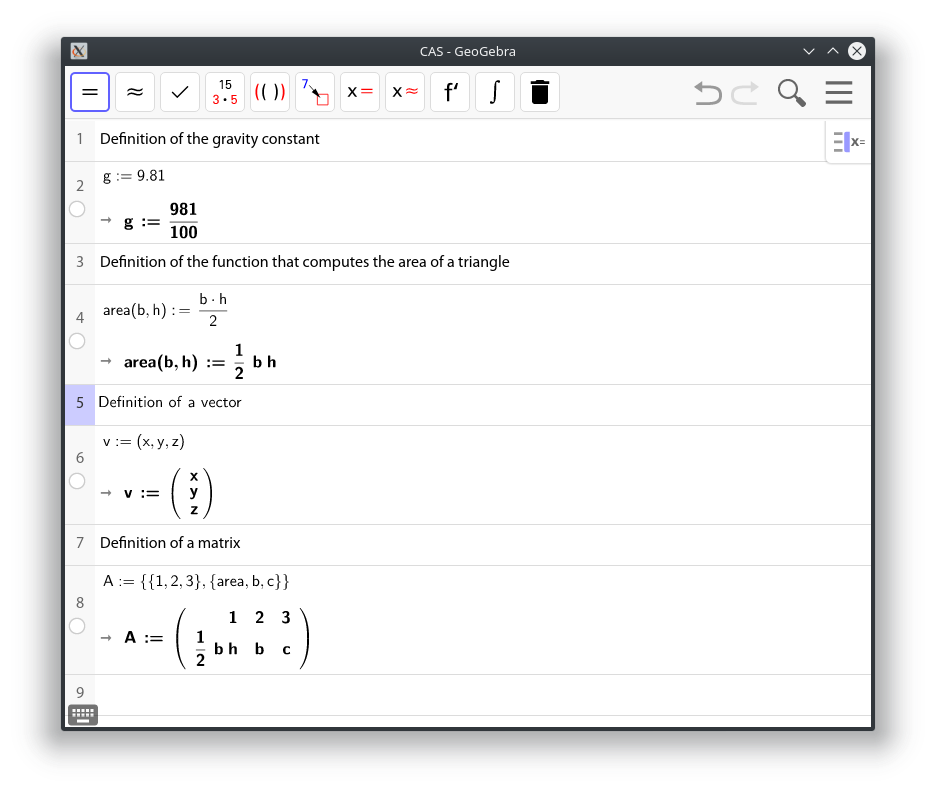
\includegraphics[scale=0.6]{img/introduction/math-expressions}
\caption{Entering mathematical expressions in the \field{Input Bar}.} \label{g:expressions}
\end{center}
\end{figure}


If we have defined a constant or function, and we change the definition after, the changes will be reflected in any other expression that contains the constant or function, except if the reference is static.

To remove a definition and free the name of the constant or function, for example \command{c}, we can use the command \command{Delete(c)} or the command \command{c:=}.


\subsection*{Predefined constants and functions}
Geogebra provides several predefined constants and functions that can be used in the mathematical expressions.
The sintax of some of these constants and functions is shown in the table~\ref{t:predefined-functions}, although, instead of using those commands, we can use the operators and constants of the virtual keyboard.

\begin{table}[h!]
\centering
\begin{tabular}{cl}
\tcrule
\textbf{Sintaxis}   & \textbf{Constante o función}                 \\
\command{pi}        & The number $\pi=3.14159\ldots$               \\
\command{Alt+e}     & Euler's constant $e=2.71828\ldots$           \\
\command{Alt+i}     & Imaginary number $i=\sqrt{-1}$               \\
\command{inf}       & Infinity $\infty$                            \\
\command{exp(x)}    & Exponential function $e^x$                   \\
\command{log(a,x)}  & Logarithmic function of base $a$, $\log_a x$ \\
\command{ln(x)}     & Neperian logarithmic function $\ln x$        \\
\command{sqrt(x)}   & Square root function $\sqrt{x}$              \\
\command{sin(x)}    & Sine function $\sin x$                       \\
\command{cos(x)}    & Cosine function $\cos x$                     \\
\command{tan(x)}    & Tangent function $\tan x$                    \\
\command{arcsin(x)} & Arcsine function $\arcsin x$                 \\
\command{arccos(x)} & Arccosine function $\arccos x$               \\
\command{arctan(x)} & Arctangent function $\arctan x$              \\
\bcrule
\end{tabular}
\caption{Sintax of some predefined constants and functions in Geogebra.} \label{t:predefined-functions}
\end{table}


\subsection*{Entering vectors and matrices}
Geogebra allows also to handle vectors and matrices.
To define a vector you must write its coordinates separated by commas between parenthesis.
For example, to enter the vector $(x,y,z)$ we have to write \command{(x,y,z)} (see figure~\ref{g:expressions}).

To define a matrix you must enter its elements by rows, separated by commas and between curly brackets.
For example, to enter the matrix
\[
\left(
\begin{array}{ccc}
1 & 2 & 3 \\
a & b & c \\
\end{array}
\right)
\]
we have to write \command{\{\{1,2,3\},\{a,b,c\}\}} (see figure~\ref{g:expressions}).


\subsection*{Simplifying expressions}
By default Geogebra always tries to simplify the mathematical expressions when it evaluates them.
For example, if you enter $x+x$ the result will be $2x$.
To avoid simplification you can change to the \button{Keep Input} mode clicking the button 
\includegraphics[scale=0.03]{img/introduction/keep-input-button}.

However, when Geogebra evaluates a mathematical expression it does not perform more complex simplifications, like, for instance, the simplification $\sin(x)^2+\cos(x)^2=1$.
To do this there are three commands:
\begin{description}
\item[Simplify] This is the most simple and tries to simplify a mathematical expression the most.
      For example, the command \command{Simplify(sin(x)\^{}2+cos(x)\^{}2)} returns \result{1}.
\item[Expand] This command tries to expand a mathematical expression computing all the possible powers, products, quotients, additions and subtractions.
      For example, the command \command{Expand((x+1)\^{}2)} returns \result{x\^{}2+2x+1}.
\item[Factor] This command tries to factorize a mathematical expression.
      For example, the command \command{Factoriza(x\^{}2+2x+1)} returns \result{(x+1)\^{}2}.
\end{description}

In any of these simplifications Geogebra uses by default the exact mode and returns fractional expressions.
To get the approximate value of a mathematical expression, with decimals, we must change to the \button{Numeric Evaluation} mode clicking the button 
\includegraphics[scale=0.03]{img/introduction/approximate-button}.
The number of decimal places showed can be set in the settings menu of Geogebra.

Lastly, it is possible to replace any variable by a value with the command \command{Substitute(<Expression>, <Substitution list>)}.
For example, the command \command{Substitute(2x+y, x=2, y=1)} returns \result{5}.


\subsection*{Entering equations and inequations}
To define equations in Geogebra the equality symbol \command{=} must be used.
Por example, the command \command{2x-y=1} defines the equation of a line.

And to define inequations we can use the symbols less than \command{<}, greater than \command{>}, less than or equal to \command{<=} or greater than or equal to \command{>=}.
For example, the command \command{x\^{}2+y\^{}2<=1} defines the circle with radius 1 centered at the origin.

To solve equations and inequation you can use the command \command{Solve(<equations>)}.
For example, the command \command{Solve(x\^{}2-5x+4=0)} returns \result{\{x=1, x=4\}}.
It is also possible to impose restrictions for the variables.
For example, the command \command{Solve(x\^{}2-5x+4=0, x>3)} returns only the solution \result{\{x=4\}}.

To solve systems of equations you must enter the list of equations separated by commans and between curly brackets.
For example, the command \command{Solve({2x+3=7, x-y=-1})} returns \result{\{x=3, y=2\}}.

This command also solves inequations.
For example, the command \command{Solve(3x-2<1)} returns \result{\{x<1\}}.


\section{Graphical representations}
One of the strengths of Geogebra is its graphics capabilities, sice it allows to represent graphically a lot of geometric objects both in the plane and in the real space.


\subsection*{Graphical representations in the real plane}
To represent geometric objects in the real plane $\mathbb{R}^2$, Geogebra uses the \field{Graphics View}.
By default any function defined in the \field{CAS View} will be plotted in this view.
To graphically represent other objects like constants, equations or inequations, it is required to click on the circle that appears to the left of the expression (see figure~\ref{g:graphics-view}).
To hide back the object in the \field{Graphics View} you have to click again on this circle.

\begin{figure}[h!]
\begin{center}
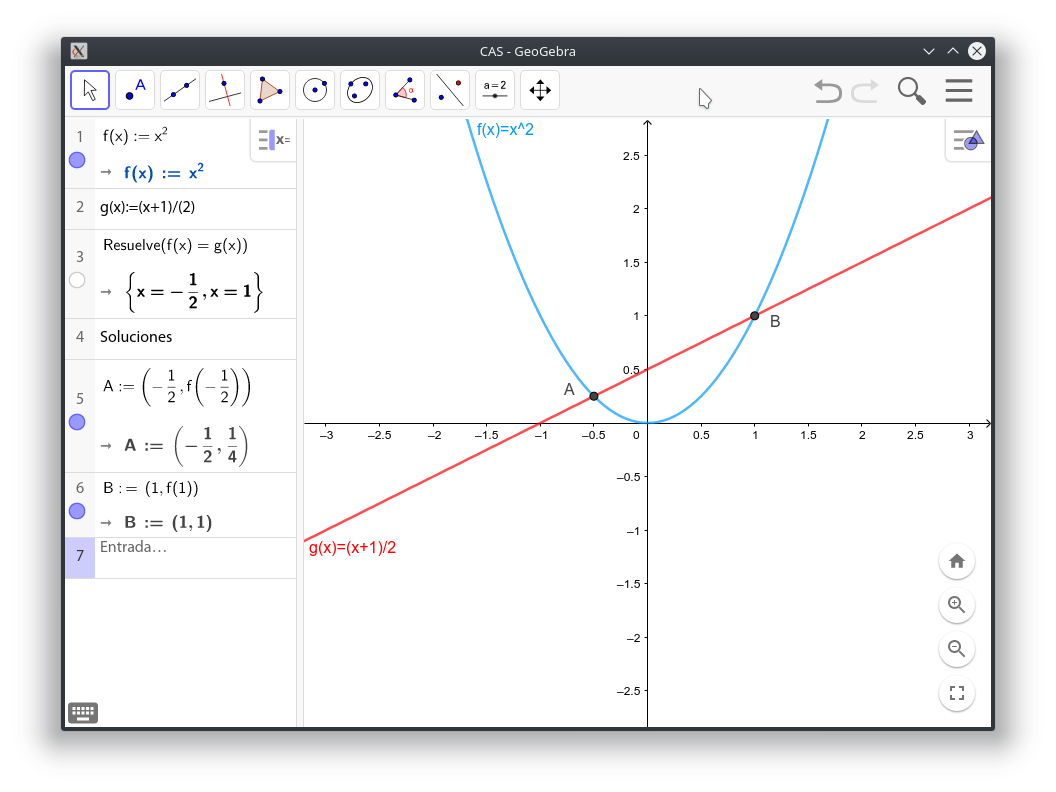
\includegraphics[width=\textwidth]{img/introduction/graphic-view}
\caption{Graphical representations in the \field{Graphics View}.} \label{g:graphics-view}
\end{center}
\end{figure}

Geogebra allows also the graphical representation of parametric functions defining the vector with the coordinate functions depending on one parameter.
For example, the command \command{g(t):=(cos(t), 2sin(t)cos(t))} plots the curve of the figure~\ref{g:parametric-curve}.

\begin{figure}[h!]
\begin{center}
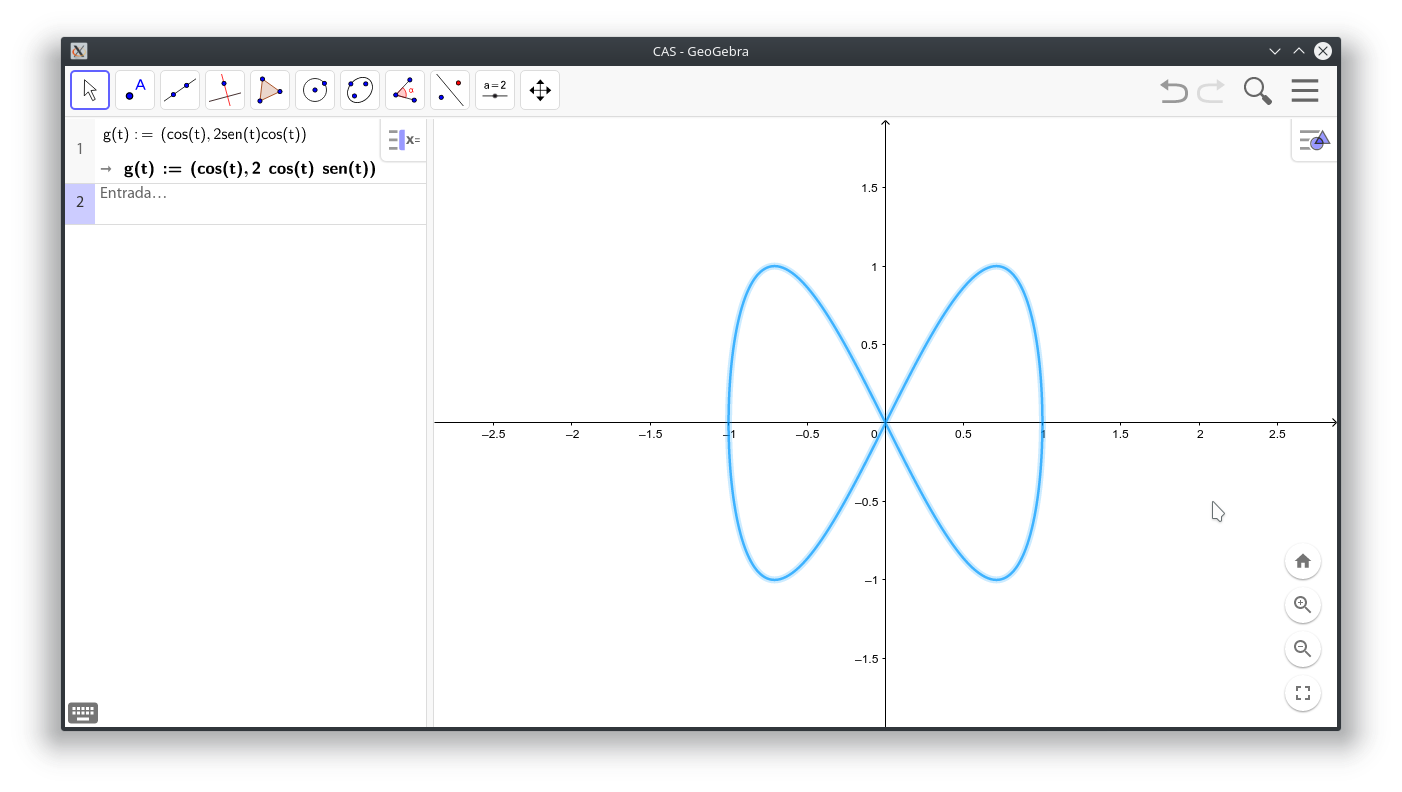
\includegraphics[width=\textwidth]{img/introduction/parametric-curve}
\caption{Graphical representation of a parametric curve in the real plane.} \label{g:parametric-curve}
\end{center}
\end{figure}

It is possible to change the aspect of any geometric object right-clicking on it and selecting the option \option{Settings} in the contextual menu that appears.
This opens a panel that allows to change the name of the object, the colour, the thickness or the opacity of the line, or even to enter a label that will appear next to the object in the \field{Graphics View}.

The \field{Graphics View} is centered at the origin of coordinates by default, but it is possible to make a zoom in or out clicking on the buttons 
\includegraphics[scale=0.03]{img/introduction/zoom-in-button} and 
\includegraphics[scale=0.03]{img/introduction/zoom-out-button} respectively.
It is also possible to move the view clicking at any position in the view and dragging the mouse.
To come back to the original view you can click on the button 
\includegraphics[scale=0.03]{img/introduction/home-button}.


\subsection*{Graphical representations in the real space}
To represent geometric objects in the real space $\mathbb{R}^3$, Geogebra uses the \field{3D Graphics View}.

By default, any function of two variables defined in the \field{CAS View} will be plotted in this view.
To graphically represent other objects like equations it is required to click on the circle that appears to the left of the expression (see figure~\ref{g:3D-graphics-view}).
Para ocultar de nuevo el objeto en la \field{Graphics View} basta con volver a hacer clic sobre ese círculo.

\begin{figure}[h!]
\begin{center}
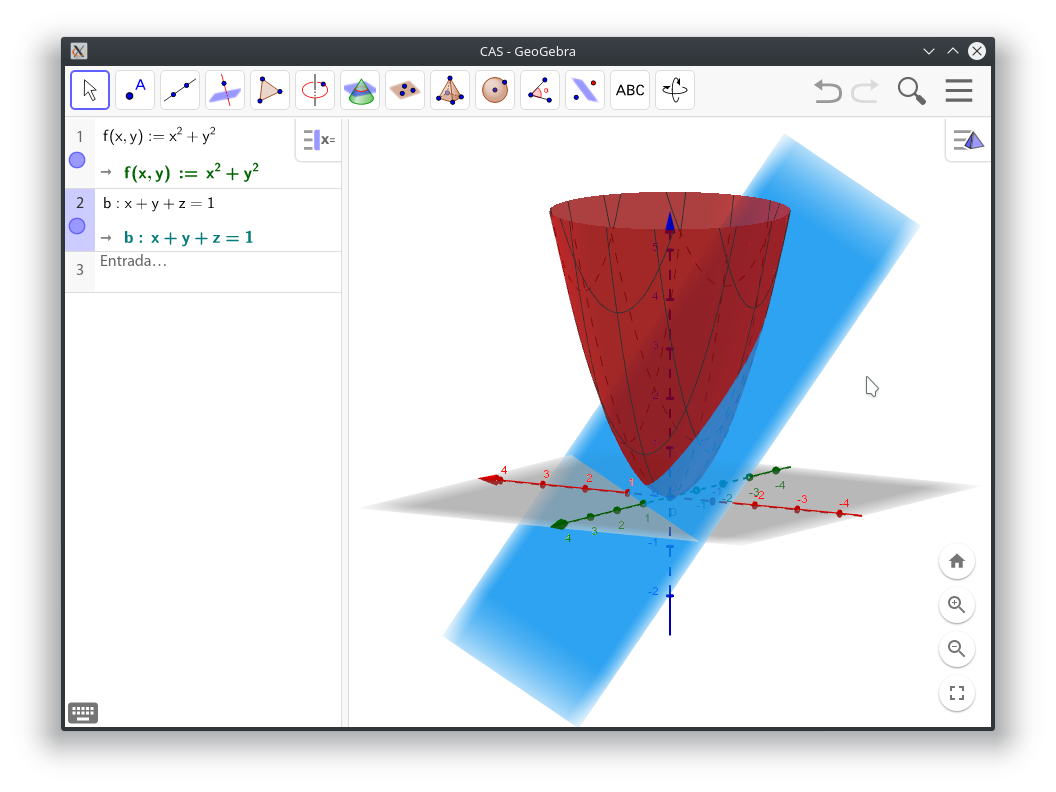
\includegraphics[width=\textwidth]{img/introduction/3D-graphic-view}
\caption{Grahpical representations in the \field{3D Graphics View}.} \label{g:3D-graphics-view}
\end{center}
\end{figure}

The same than in the \field{Graphics View} it is also possible to represent parametric functions defining the vector with the coordinate functions depending on one parameter.
For example, the command \command{h(t):=(cos(t), sin(t), t/2)} plots the curve of figure~\ref{g:3D-parametric-curve}.

\begin{figure}[h!]
\begin{center}
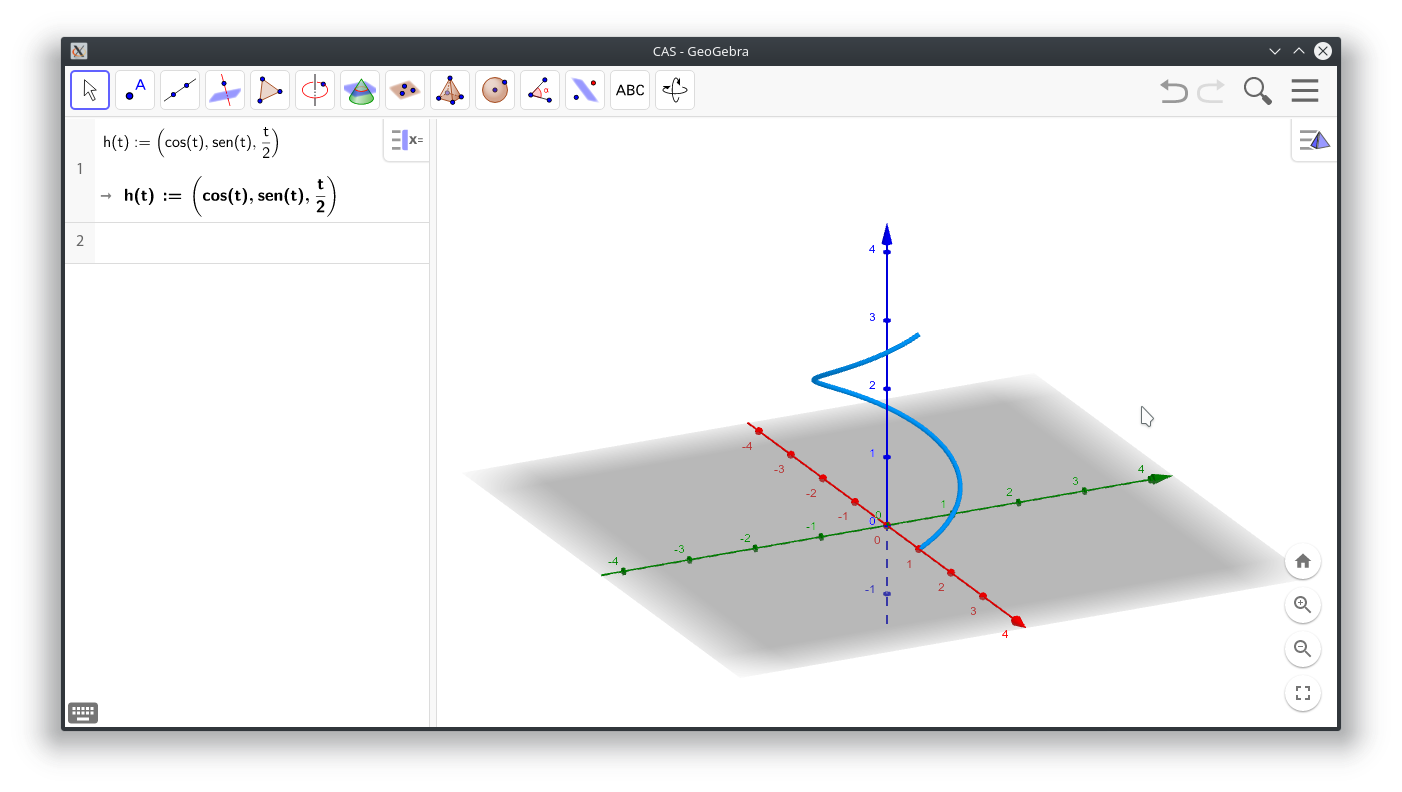
\includegraphics[width=\textwidth]{img/introduction/3D-parametric-curve}
\caption{Graphical representation of a parametric curve in the real space.} \label{g:3D-parametric-curve}
\end{center}
\end{figure}

The same than in the \field{Graphics View}, it is possible to change the aspect of any geometric object right-clicking on it and selecting the option \option{Settings} in the contextual menu that appears.
This opens a panel that allows to change the name of the object, the colour, the thickness or the opacity of the line, or even to enter a label that will appear next to the object in the \field{3D Graphics View}.

In the same way, it is possible to make a zoom in or out clicking on the buttons 
\includegraphics[scale=0.03]{img/introduction/zoom-in-button} and 
\includegraphics[scale=0.03]{img/introduction/zoom-out-button} respectively.
It is also possible to move the view with the button 
\includegraphics[scale=0.03]{img/introduction/move-button} or to rotate it with the button 
\includegraphics[scale=0.03]{img/introduction/rotate-button}.


\section{File management}
The mathematical expressions and calculus of the \field{CAS View} and the graphics of the \field{Graphics View} and \field{3D Graphics View} can be saved into a file.

\subsection*{Saving a file}
To save the mathematical expressions, calculus and graphics of a working session you must select the menu \menu{File>Save}.
If you have not logged in to the Geogebra web site a dialog appears asking for the user name an password to log in (see figure~\ref{g:login}).
If the you has no account in this site now is possible to register, but if you do not want to log in just click the link \button{Continue without signing in now}.

\begin{figure}[h!]
\begin{center}
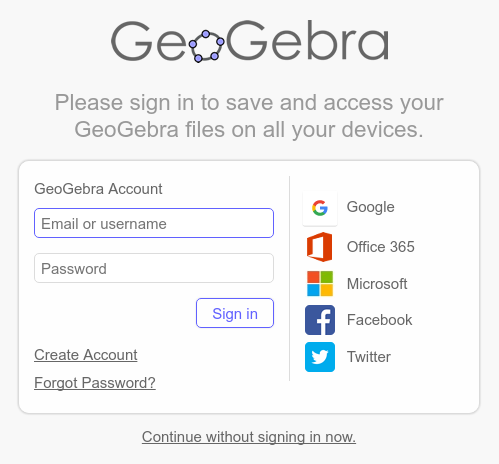
\includegraphics[scale=0.6]{img/introduction/login}
\caption{Login dialog of Geogebra web site.} \label{g:login}
\end{center}
\end{figure}

If you have logged in to the Geogebra web site, it will ask for the file name and the file will be uploaded to the Geogebra web site.
This way the file will be available whenever we are connected to this site with our user account.

If you have not logged in to the Geogebra web site, then a dialog is shown where you can enter the file name and select the local folder where to save the file in your computer.
Geogebras' files have extension \texttt{*.ggb}.

Once the file is saved, its name will appear in the title bar of the Geogebra window.


\subsubsection*{Opening a file}
To open a file in Geogebra you can use the menu \menu{File>Open}.
In the dialog shown you can choose to open a file from the Geogebra web site or to open a local file.

If you has logged in to the Geogebra web site, the files saved in our user account will appear automatically.
Eve if you are not logged in, you can open any public file in the Geogebra cloud.
For that we can search for a file entering a keyword in the search bar and Geogebra will show a list with all the files that contains that word.
Selecting any of them will download the file and open it.

If you want to open a local file you have to click on the folder icon.
This will open a dialog where you can select the file to open.


% \section{Printing}
% Geogebra permite imprimir las vistas gráficas seleccionando el menú \menu{Previsualización}.
% Tras esto aparece un cuadro de diálogo donde se puede seleccionar la ventana gráfica que se desea imprimir and las unidades de los ejes.
% Finalmente aparece el cuadro de diálogo de las impresoras donde hay que seleccionar la impresora con la que se quiere imprimir.

% También es posible exportar las vistas gráficas a diferentes formatos con el menú \menu{Descargar como}.
% Si se desea imprimir además de las gráficos las expresiones de la \field{CAS View} hay que seleccionar la opción \option{Construcción dinámica con página web (html)}.
% Esto genera una página web que puede abrirse con cualquier navegador and después imprimirse de la forma habitual.


\section{Solved exercises}
\begin{enumerate}
\item Enter and evaluate the following expressions.
      \begin{enumerate}
      \item $4x-\dfrac{1}{x}-5$.
            \begin{indication}
            Enter the expression \command{4x-1/x-5} in the \field{Input Bar} of the \field{CAS View}.
            \end{indication}
      \item $\dfrac{4x-1}{x}-5$.
            \begin{indication}
            Enter the expression \command{(4x-1)/x-5} in the \field{Input Bar} of the \field{CAS View}.
            \end{indication}
      \item $4x-\dfrac{1}{x-5}$.
            \begin{indication}
            Enter the expression \command{4x-1/(x-5)} in the \field{Input Bar} of the \field{CAS View}.
            \end{indication}
      \item $\dfrac{4x-1}{x-5}$.
            \begin{indication}
            Enter the expression \command{(4x-1)/(x-5)} in the \field{Input Bar} of the \field{CAS View}.
            \end{indication}
      \end{enumerate}

\item Define the following mathematical objects and plot them.
      \begin{enumerate}
      \item The constants $a=2$ and $b=3$.
            \begin{indication}
            \begin{enumerate}
            \item Enter the command \command{a:=2} in the \field{Input Bar} of the \field{CAS View} and activate the \field{Graphics View}.
            \item To plot the slider of the constant click the circle that appears to the left of the previous expression.
            \item Enter the command \command{b:=3} in the \field{Input Bar}.
            \item To plot the slider of the constant click the circle that appears to the left of the previous expression.
            \end{enumerate}
            \end{indication}
      \item The line $f(x)=a+bx$.
            Use the sliders of the constants to see how the line changes.
            \begin{indication}
            Enter the command \command{f(x):=a+b*x} in the \field{Input Bar}.
            \end{indication}
      \item The equation $ax^2+by^2=8$.
            Use the sliders of the constants to see how the conic changes.
            \begin{indication}
            Enter the command \command{a*x\^{}2+b*y\^{}2=8} in the \field{Input Bar}.
            \end{indication}
      \end{enumerate}

\item Define the following functions and plot them.
      \begin{enumerate}
      \item $f(x):=x^2$.
            \begin{indication}
            Enter the command \command{f(x):=x\^{}2} in the \field{Input Bar} of the \field{CAS View} and activate the \field{Graphics View}.
            \end{indication}
      \item $g(x):=\log(x)$.
            \begin{indication}
            Enter the command \command{g(x):=log(x)} in the \field{Input Bar}.
            \end{indication}
      \item $h(x):=\sin(x)$.
            \begin{indication}
            Enter the command \command{g(x):=sin(x)} in the \field{Input Bar}.
            \end{indication}
      \item $g\circ f(x)$.
            \begin{indication}
            Enter the command \command{g(f(x))} in the \field{Input Bar} and click the circle that appears to the left of the expression.
            \end{indication}
      \item $h\circ g \circ f(x)$.
            \begin{indication}
            Enter the command \command{h(g(f(x)))} in the \field{Input Bar} and click the circle that appears to the left of the expression.
            \end{indication}
      \item $f\circ g \circ h(x)$.
            \begin{indication}
            Enter the command \command{f(g(h(x)))} in the \field{Input Bar} and click the circle that appears to the left of the expression.
            \end{indication}
      \end{enumerate}

\item Given the matrices
      \[
      A=\left(
      \begin{array}{cc}
      a_{11} & a_{12} \\
      a_{21} & a_{22} \\
      a_{31} & a_{32}
      \end{array}
      \right)
      \qquad
      B=\left(
      \begin{array}{ccc}
      1 & 2 & 3 \\
      4 & 5 & 6
      \end{array}
      \right)
      \]
      and the vector $\mathbf{v}=(x, y, z)$, se pide:

      \begin{enumerate}
      \item Define the matrices $A$ and $B$, and the vector $v$.
            \begin{indication}
            \begin{enumerate}
            \item Enter the command \command{A:=\{\{a\_{11},a\_{12}\},\{a\_{21},a\_{22}\},\{a\_{31},a\_{32}\}\}} in the \field{Input Bar} of the \field{CAS View}.
            \item Enter the command \command{B:=\{\{1,2,3\},\{4,5,6\}\}} in the \field{Input Bar}.
            \item Enter the command \command{v:=(x,y,z)} in the \field{Input Bar}.
            \end{enumerate}
            \end{indication}
      \item Compute $A\cdot B$.
            \begin{indication}
            Enter the command \command{A*B} in the \field{Input Bar}.
            \end{indication}
      \item Compute $B\cdot A$.
            \begin{indication}
            Enter the command \command{B*A} in the \field{Input Bar}.
            \end{indication}
      \item Compute $\mathbf{v}\cdot A$.
            \begin{indication}
            Enter the command \command{v*A} in the \field{Input Bar}.
            \end{indication}
      \item Compute $B\cdot \mathbf{v}$.
            \begin{indication}
            Enter the command \command{B*v} in the \field{Input Bar}.
            \end{indication}
      \item Substitute $x=1$, $y=1$ and $z=0$ in the previous vector and plot it.
            \begin{indication}
            Enter the command \command{Substitute(\$,\{x=1,y=1,z=0\})} in the \field{Input Bar} and click the circle that appears to the left of the expression.
            \end{indication}
      \item Compute the modulus of the previous vector.
            \begin{indication}
            Enter the command \command{|\$|} in the \field{Input Bar} and click the circle that appears to the left of the expression.
            \end{indication}
      \item Change the previous substitution for $x=0$, $y=0$ and $z=1$ and observe how changes the modulus of the previous vector.
            \begin{indication}
            Edit the line with the substitution and change it for \command{Substitute(\$,\{x=0,y=0,z=1\})} in the \field{Input Bar}.
            \end{indication}
      \end{enumerate}

\item Find out the points where the graphs of the functions $f(x)=x^2$ and $g(x)=\dfrac{x+1}{2}$ intersect and plot them.
      \begin{enumerate}
      \item Enter the command \command{f(x):=x\^{}2} in the \field{Input Bar} of the \field{CAS View} and activate the \field{Graphics View}.
      \item Enter the command \command{g(x):=(x+1)/2} in the \field{Input Bar}.
      \item To solve the equation, enter the command \command{Solve(f=g)} in the \field{Input Bar}.
      \item To plot the intersection points, enter the command \command{Intersect(f,g)} in the \field{Input Bar} and click on the circle that appears to the left of the expression.
      \end{enumerate}

\item Plot the parametric function
      \[
      g(t)=
      \begin{cases}
      \cos(t) \\
      2\sin(t)\cos(t)
      \end{cases}
      t\in \mathbb{R}
      \]

      \begin{indication}
      Enter the command \command{g(t):=(cos(t), 2sin(t)cos(t))} in the \field{Input Bar} of the \field{CAS View} and activate the \field{Graphics View}.
      \end{indication}

\item Plot the following surfaces
      \[
      f(x,y)=\dfrac{2\sin(x^2+y^2)}{\sqrt{x^2+y^2}}, \qquad x^2+y 2+(z-2)^2=1
      \]
      and and the parametric curve
      \[
      h(t)=
      \begin{cases}
      \sin(t) \\
      \cos(t) \\
      t/2
      \end{cases}
      t\in \mathbb{R}
      \]
      \begin{indication}
      \begin{enumerate}
      \item Enter the command \command{f(x,y):=2sin(x\^{}2+y\^{}2)/sqrt(x\^{}2+y\^{}2)} in the \field{Input Bar} of the \field{CAS View} and activate the \field{3D Graphics View}.
      \item Enter the command \command{x\^{}2+y\^{}2+(z-2)\^{}2=1}  in the \field{Input Bar}.
      \item Enter the command \command{h(t):=(sin(t),cos(t),t/2)}  in the \field{Input Bar}.
      \end{enumerate}
      \end{indication}
\end{enumerate}
% !TEX root = ../practicas_geogebra.tex
% Author: Alfredo Sánchez Alberca (asalber@ceu.es)
\chapter{Elementary functions}

% \section{Fundamentos teóricos}

% En esta práctica se introducen los conceptos básicos sobre funciones reales de variable real, esto es, funciones
% \[f:\mathbb{R}\rightarrow \mathbb{R}.\]

% \subsection{Dominio e imagen}

% El \emph{Dominio} de la función $f$ es el conjunto de los números reales $x$ para los que existe $f(x)$ y se designa mediante $\dom f$.

% La \emph{Imagen} de $f$ es el conjunto de los números reales $y$ para los que existe algún $x\in \mathbb{R}$ tal que $f(x)=y$, y se denota por $\im f$.


% \subsection{Signo y crecimiento}
% El \emph{signo} de la función es positivo $(+)$ en los valores de $x$ para los que $f(x)>0$ y negativo $(-)$ en los que $f(x)<0$.
% Los valores de $x$ en los que la función se anula se conocen como \emph{raíces} de la función.

% Una función $f(x)$ es \emph{creciente} en un intervalo $I$ si $\forall\, x_1, x_2 \in I$ tales que $x_1<x_2$ se verifica que $f(x_1)\leq f(x_2)$.

% Del mismo modo, se dice que una función $f(x)$ es \emph{decreciente} en un intervalo $I$ si $\forall\, x_1, x_2 \in I$ tales que $x_1<x_2$ se verifica que $f(x_1)\geq f(x_2)$. En la figura~\ref{g:crecimiento} se muestran estos conceptos.

% \begin{figure}[h!]
% 	\centering \subfigure[Función creciente.] {\label{g:funcion_creciente}
% 		\scalebox{1}{\input{img/funciones_elementales/funcion_creciente}}}\qquad
% 	\subfigure[Función decreciente.]{\label{g:funcion_decreciente}
% 		\scalebox{1}{\input{img/funciones_elementales/funcion_decreciente}}}
% 	\caption{Crecimiento de una función.}
% 	\label{g:crecimiento}
% \end{figure}


% \subsection{Extremos Relativos}
% Una función $f(x)$ tiene un \emph{máximo relativo} en $x_0$ si existe un entorno $A$ de $x_0$ tal que $\forall x \in A$
% se verifica que $f(x)\leq f(x_0)$.

% Una función $f(x)$ tiene un \emph{mínimo relativo} en $x_0$ si existe un entorno $A$ de $x_0$ tal que $\forall x\in A$
% se verifica que $f(x)\geq f(x_0)$.

% Diremos que la función $f(x)$ tiene un \emph{extremo relativo} en un punto si tiene un \emph{máximo o mínimo relativo}
% en dicho punto. Estos conceptos se muestran en la figura~\ref{g:extremos}.

% \begin{figure}[h!]
% 	\centering \subfigure[Máximo relativo.] {\label{g:maximo}
% 		\scalebox{1}{\input{img/funciones_elementales/maximo}}}\qquad
% 	\subfigure[Mínimo relativo.]{\label{g:minimo}
% 		\scalebox{1}{\input{img/funciones_elementales/minimo}}}
% 	\caption{Extremos relativos de una función.}
% 	\label{g:extremos}
% \end{figure}

% Una función $f(x)$ está \emph{acotada superiormente} si $\exists K\in\mathbb{R}$ tal que $f(x)\leq K$ $\forall x \in \dom f$. Análogamente, se dice que una función $f(x)$ está \emph{acotada inferiormente} si $\exists K\in\mathbb{R}$ tal que $f(x)\geq K$ $\forall x \in \dom f$.

% Una función $f(x)$ está \emph{acotada} si lo está superior e inferiormente, es decir si $\exists K\in\mathbb{R}$ tal que $|f(x)|\leq K$ $\forall x \in \dom f$.


% \subsection{Concavidad}

% De forma intuitiva se puede decir que una función $f(x)$ es \emph{cóncava} en un intervalo $I$ si $\forall\, x_1, x_2
% \in I$, el segmento de extremos $(x_1,f(x_1))$ y $(x_2,f(x_2))$ queda por encima de la gráfica de $f$.

% Análogamente se dirá que es \emph{convexa} si el segmento anterior queda por debajo de la gráfica de $f$.

% Diremos que la función $f(x)$ tiene un \emph{punto de inflexión} en $x_0$ si en ese punto la función pasa de cóncava a
% convexa o de convexa a cóncava. Estos conceptos se ilustran en la figura~\ref{g:concavidad}.

% \begin{figure}[h!]
% 	\centering \subfigure[Función cóncava.] {\label{g:funcion_convexa}
% 		\scalebox{1}{\input{img/funciones_elementales/funcion_convexa}}}\qquad
% 	\subfigure[Función convexa.]{\label{g:funcion_concava}
% 		\scalebox{1}{\input{img/funciones_elementales/funcion_concava}}}
% 	\caption{Concavidad de una función.}
% 	\label{g:concavidad}
% \end{figure}

% \subsection{Asíntotas}

% La recta $x=a$ es una \emph{asíntota vertical} de la función $f(x)$ si al menos uno de los límites laterales de $f(x)$ cuando $x$ tiende hacia $a$ es $+\infty$ o $-\infty$, es decir cuando se verifique alguna de las siguientes igualdades
% \[
% 	\ \lim_{x\rightarrow a^{+}}f(x)=\pm\infty   \quad \textrm{o} \quad
% 	\lim_{x\rightarrow a^{-}}f(x)=\pm\infty
% \]

% La recta $y=b$ es una \emph{asíntota horizontal} de la función $f(x)$ si alguno de los límites de $f(x)$ cuando $x$ tiende hacia $+\infty$ o $-\infty$ es igual a $b$, es decir cuando se verifique
% \[
% 	\ \lim_{x\rightarrow -\infty }f(x)=b    \quad \textrm{o} \quad
% 	\ \lim_{x\rightarrow +\infty }f(x)=b
% \]

% La recta $y=mx+n$ es una \emph{asíntota oblicua} de la función $f(x)$ si alguno de los límites de $f(x)-(mx+n)$ cuando $x$ tiende hacia $+\infty$ o $-\infty$ es igual a 0, es decir si

% \[
% 	\ \lim_{x\rightarrow -\infty }{(f(x)-mx)}=n    \quad \textrm{o} \quad
% 	\ \lim_{x\rightarrow +\infty }{(f(x)-mx)}=n
% \]

% En la figura~\ref{g:asintotas} se muestran los distintos tipos de asíntotas.

% \begin{figure}[h!]
% 	\centering \subfigure[Asíntota horizontal y vertical.] {\label{g:asintotahorizontalyvertical}
% 		\scalebox{1}{\input{img/funciones_elementales/asintota_vertical}}}\qquad\qquad
% 	\subfigure[Asíntota vertical y oblicua.]{\label{g:asintotaoblicua}
% 		\scalebox{1}{\input{img/funciones_elementales/asintota_oblicua}}}
% 	\caption{Tipos de asíntotas de una función.}
% 	\label{g:asintotas}
% \end{figure}


% \subsection{Periodicidad}
% Una función $f(x)$ es \emph{periódica} si existe $h\in\mathbb{R^{+}}$ tal que \[f(x+h)=f(x)\  \forall x\in \dom f\] siendo el período $T$ de la función, el menor valor $h$ que verifique la igualdad anterior.

% En una función periódica, por ejemplo $f(x)=A\sin(wt)$, se denomina \emph{amplitud} al valor de $A$, y es la mitad de la diferencia entre los valores máximos y mínimos de la función. En la figura~\ref{g:periodoyamplitud} se ilustran estos conceptos.

% \begin{figure}[h!]
% 	\centering
% 	\scalebox{0.8}{\input{img/funciones_elementales/funcion_periodica}}
% 	\caption{Periodo y amplitud de una función periódica.}
% 	\label{g:periodoyamplitud}
% \end{figure}

% \clearpage
% \newpage

\section{Solved exercises}

\begin{enumerate}[leftmargin=*]
\item Consider the function
      \[
      f(t)=\frac{t^{4} +19t^{2} - 5}{t^{4} +9t^{2} - 10}.
      \]

      Representarla gráficamente y determinar a partir de dicha representación:

      \begin{enumerate}
      \item  Domain.
            \begin{indication}
            \begin{enumerate}
            \item Enter the expression \command{(t\^{}4+19t\^{}2-5)/(t\^{}4+9t\^{}2-10)} in the \field{Input Bar} of the \field{Vista CAS View} and activate the \field{Graphics View}.
            \item To determine the domain look at the values of $x$ where the function does exists, that is, where there is graph.
            \item Remember that, for this and the other parts of this exercise, we pretend to get approximate conclusions looking at the graph of the function.
            \end{enumerate}
            \end{indication}

      \item Image.
            \begin{indication}
            Look at the values of $y$ that are output of the function, that is, where there is graph.
            \end{indication}

      \item Asymtotes.
            \begin{indication}
            Look at the lines (horizontal, vertical or oblique) where the graph approaches (the distance between the graph and the line tends to zero as they tend to infinity).
            \end{indication}

      \item  Roots.
            \begin{indication}
            Look at the values of $x$ where the graph cuts the horizontal axis.
            \end{indication}

      \item Sign.
            \begin{indication}
            Look at the values of $x$ where the graph is over the horizontal axis (positive) and where it is under the horizontal axis (negative).

            \end{indication}

      \item Growth.
            \begin{indication}
            Look at the values of $x$ where $y$ increases when $x$ increases (increasing) and the values where $y$ decreases when $x$ increases (decreasing).
            \end{indication}

      \item Concavity.
            \begin{indication}
            Look at the values of $x$ where the curvature of the graph is up $\cup$ (concave up or convex) and where the curvature is $\cap$ (concave down or simply concave).
            \end{indication}

      \item Local extrema.
            \begin{indication}
            Look at the values of $x$ where the graph has a peak (relative maximum) and where the graph has a valley (relative minimum).
            \end{indication}

      \item Inflection points.
            \begin{indication}
            Look at the values of $x$ where the curvature changes continuously.
            \end{indication}
      \end{enumerate}

\item Representar en una misma gráfica las funciones $2^{x}, e^{x}, 0.7^{x}, 0.5^{x}$.
      A la vista de las gráficas obtenidas, ¿para qué valores de $a$ será la función creciente? ¿Y para qué valores de $a$ será decreciente?
      \begin{indication}
      \begin{enumerate}
      \item Introducir la función \command{2\^{}x} en la in the \field{Input Bar} of the \field{Vista CAS View}.
      \item Introducir la función \command{e\^{}x} en la \field{Barra de Entrada}.
      \item Introducir la función \command{0.7\^{}x} en la \field{Barra de Entrada}.
      \item Introducir la función \command{0.5\^{}x} en la \field{Barra de Entrada}.
      \item La función exponencial $a^x$ será creciente cuando $a>1$ y decreciente cuando $0<a<1$.
      \end{enumerate}
      \end{indication}

\item Representar en una misma gráfica las funciones siguientes, indicando su período y amplitud.
      \begin{enumerate}
      \item $\sin{x}$, $\sin{x}+2$, $\sin{(x+2)}$.
      \item $\sin{2x}$, $2\sin{x}$, $\sin\frac{x}{2}$.
            \begin{indication}
            \begin{enumerate}
            \item Introducir la función \command{sen(x)} en la in the \field{Input Bar} of the \field{Vista CAS View}.
            \item Introducir la función \command{sen(x)+2} en la \field{Barra de Entrada}.
            \item Introducir la función \command{sen(x+2)} en la \field{Barra de Entrada}.
            \item Introducir la función \command{sen(2x)} en la \field{Barra de Entrada}.
            \item Introducir la función \command{2sen(x)} en la \field{Barra de Entrada}.
            \item Introducir la función \command{sen(x/2)} en la \field{Barra de Entrada}.
            \end{enumerate}
            \end{indication}
      \end{enumerate}


\item Representar en una gráfica la función
      \[
      \ f(x)=\left\{
      \begin{array}{cl}
      -2x   & \hbox{si $x\leq0$;} \\
      x^{2} & \hbox{si $x>0$.}    \\
      \end{array}
      \right.
      \]

      \begin{indication}
      Introducir la función \command{Si(x<=0, -2x, x\^{}2)} en la \field{Barra de Entrada}.
      \end{indication}
\end{enumerate}


\section{Ejercicios propuestos}
\begin{enumerate}[leftmargin=*]
\item Hallar el dominio de las siguientes funciones a partir de sus representaciones gráficas:

      \begin{enumerate}
      \item $f(x)=\dfrac{x^{2} + x + 1}{x^{3} - x}$
      \item $g(x)=\sqrt[2]{x^{4}-1}$.
      \item $h(x)=\cos{\dfrac{x + 3}{x^{2} + 1}}$.
      \item $l(x)=\arcsin{\dfrac{x}{1+x}}$.
      \end{enumerate}

\item Se considera la función
      \[
      \ f(x)=\frac{x^{3} + x +2}{5x^{3} - 9x^{2} - 4x + 4}.
      \]

      Representarla gráficamente y determinar a partir de dicha representación:

      \begin{enumerate}
      \item Dominio.
      \item Imagen.
      \item Asíntotas.
      \item Raíces.
      \item Signo.
      \item Intervalos de crecimiento y decrecimiento.
      \item Intervalos de concavidad y convexidad.
      \item Extremos relativos.
      \item Puntos de inflexión.
      \end{enumerate}

\item Representar en una misma gráfica las funciones $\log_{10}{x}$, $\log_{2}{x}$, $\log{x}$, $\log_{0.5}{x}$.
      \begin{enumerate}
      \item A la vista de las gráficas obtenidas, indicar cuáles de las funciones anteriores son crecientes y cuáles son decrecientes.
      \item Determinar, a partir de los resultados obtenidos, o representando nuevas funciones si fuera necesario, para qué valores de $a$ será
            creciente la función $\log_{a}{x}$.
      \item Determinar, a partir de los resultados obtenidos, o representando nuevas funciones si fuera necesario, para qué valores de $a$ será
            decreciente la función $\log_{a}{x}$.
      \end{enumerate}

\item Completar las siguientes frases con la palabra igual, o el número de veces que sea mayor o menor en cada caso:
      \begin{enumerate}
      \item La función $\cos{2x}$ tiene un período............ que la función $\cos{x}$.
      \item La función $\cos{2x}$ tiene una amplitud............ que la función $\cos{x}$.
      \item La función $\cos\dfrac{x}{2}$ tiene un período............ que la función $\cos{3x}$.
      \item La función $\cos\dfrac{x}{2}$ tiene una amplitud............ que la función $\cos{3x}$.
      \item La función $3\cos{2x}$ tiene un período............ que la función $\cos\dfrac{x}{2}$.
      \item La función $3\cos{2x}$ tiene una amplitud............ que la función $\cos\dfrac{x}{2}$.
      \end{enumerate}

\item Hallar a partir de la representación gráfica, las soluciones de $e^{-1/x}=\dfrac{1}{x}$.

\item Representar en una gráfica la función
      \[
      \ f(x)=\left\{
      \begin{array}{ll}
      x^{3}   & \hbox{si $x<0$}    \\
      e^{x}-1 & \hbox{si $x\geq0$} \\
      \end{array}
      \right.
      \]

\end{enumerate}

% \include{chapters/limites_continuidad}
% \include{chapters/derivadas_una_variable}
% \include{chapters/polinomios_taylor}
% \include{chapters/derivadas_implicitas_parametricas}
% \include{chapters/integrales}
% \include{chapters/primitivas}
% \include{chapters/integral_riemann}
% \include{chapters/ecuaciones_diferenciales}
% \include{chapters/derivadas_n_variables}
\end{document}
